\documentclass[10pt,conference,compsocconf]{IEEEtran}
\usepackage[english]{babel}
\usepackage[ruled]{algorithm}
\usepackage{algpseudocode}
\usepackage{color}
\let\labelindent\relax
\usepackage{enumitem}
\let\proof\relax
\let\endproof\relax 
\usepackage{amsthm}
\usepackage[cmex10]{amsmath}
\usepackage{amsfonts}
\usepackage{multicol}
\usepackage[font=small]{subcaption}
\usepackage{graphicx}
\usepackage[hidelinks,bookmarks=false,pdfpagelabels]{hyperref}

% definition environment
\newtheorem{definition}{Definition}
\newtheorem{theorem}{Theorem}
\newtheorem{lemma}{Lemma}
\newtheorem{invariant}{Invariant}

% typewriter font family that support hyphenation
%\newcommand\textvtt[1]{{\normalfont\fontfamily{cmvtt}\selectfont #1}}
\hyphenation{MD-List} 
\hyphenation{skip-list}
\hyphenation{De-le-te-Min}

\algtext*{EndWhile}
\algtext*{EndFor}
\algtext*{EndIf}
\algtext*{EndFunction}
\newcommand\NIL{\text{NIL}}
\newcommand\TRUE{\text{\textbf{true}}}
\newcommand\FALSE{\text{\textbf{false}}}
\newcommand\BREAK{\text{\textbf{break}}}
\newcommand\CONTINUE{\text{\textbf{continue}}}
\newcommand\AND{\;\text{\textbf{and}}\;}
\newcommand\OR{\;\text{\textbf{or}}\;}
\algrenewcommand\algorithmicindent{1em}

\algblockdefx[StructBlock]{Struct}{EndStruct} [1]{\textbf{struct} #1} [0]{}
\algtext*{EndStruct}
\algblockdefx[ClassBlock]{Class}{EndClass} [1]{\textbf{class} #1} [0]{}
\algtext*{EndClass}
\algblockdefx[MacroBlock]{Define}{EndDefine} [2]{\textbf{define} #1(#2)} [0]{}
\algtext*{EndDefine}
\algblockdefx[InlineBlock]{Inline}{EndInline} [2]{\textbf{inline function} \textsc{#1}(#2)} [0]{}
\algtext*{EndInline}

\begin{document}

\title{An Efficient Lock-free Logarithmic Search Data Structure Based on Multi-dimensional List}


\author{\IEEEauthorblockN{Deli~Zhang\hspace{14pt} Damian~Dechev}
    \IEEEauthorblockA{Department of Computer Science\\
        University of Central Florida\\
        Orlando, FL 32817, USA\\
    de-li.zhang@knights.ucf.edu \hspace{14pt} dechev@cs.ucf.edu}
}

\maketitle

\begin{abstract}
    Logarithmic search data structures, such as search trees and skiplists, are fundamental building blocks of many applications.
    Although the self-balancing binary search trees are among the most ubiquitous sequential search data structures, designing non-blocking rebalancing algorithms is challenging due to the required structural alternation, which may stall other concurrent operations.
    Skiplists, which probabilistically create multiple levels of shortcuts in an ordered list, provide practical alternatives to balanced search trees.
    The use of skiplists eliminates the need of rebalancing and ensures amortized logarithmic sequential search time, but concurrency is limited under write-dominated workload because the linkage updating process involves multiple nodes.
    
    In this paper, we present a linearizable lock-free dictionary design based on a multi-dimensional list (MDList).
    A node in an MDList arranges its child nodes by their dimensionality and order them by coordinate prefix. 
    The search operation works by first generating a one-to-one mapping from the scalar keys to a high-dimensional vectors space, then uniquely locating the target position by using the vector as coordinates.
    Our algorithm guarantees worst-case search time of $\mathcal{O}(\log N)$ where $N$ is the size of key space.
    Moreover, the ordering property of the data structure is readily maintained during mutations without rebalancing nor randomization. 
    In our experimental evaluation using a micro-benchmark, our dictionary outperforms the state of the art approaches by as much as $100\%$ when the key universe is large and an average of $30\%$ across all scenarios.
\end{abstract}

\begin{IEEEkeywords}
    Concurrent Data Structure, Dictionary, Lock-free, Multi-dimensional List, Search Tree, Skiplist
\end{IEEEkeywords}

\section{Introduction}\label{sec:intro}
Non-blocking data structures are pivotal to leverage the performance of parallel applications on current multi-core and future many-core systems.
Recent years have seen rising interests in the concurrent logarithmic search data structures that implement the \emph{dictionary} abstract data type.
A dictionary stores a set of key-value pairs where the keys are drawn from a totally ordered universe. 
It is defined only by its semantics that specify three canonical operations: \textsc{Insert} which adds a key-value pair, \textsc{Delete} which removes the value associated with a specific key, and \textsc{Find} which returns the associated value if the specific key is in the set.
In-memory dictionaries can be implemented on top of either binary search trees (BSTs) or skiplists~\cite{pugh1990skip}. 

Binary search trees are among the most ubiquitous sequential data structures. 
Despite recent research efforts, designing a self-balancing non-blocking BST is challenging and remains an active topic~\cite{brown2014general,natarajan2014fast,ellen2014amortized}.
One difficulty is to devise a correct and scalable design for predecessor query, which serves as the subroutine for all three operations to locate the physical node containing the target key.
When executing the predecessor query concurrently with write operations, the physical location of the target key in the tree might have changed before the search finishes.
This is especially troublesome when a predecessor query fails to reach the target node, under which circumstance it has to decide whether the target element is absent, or the target element's physical location has been changed by some concurrent updates~\cite{drachsler2014practical}. 
The problem stems from the lack of one-to-one mapping between the \emph{logical ordering} of keys and the physical layout of a BST.
For example, the BST in Figure~\ref{fig:bst1} and~\ref{fig:bst2} differ in layout but represent the same ordering for integers $\{1,6,7\}$.
If a predecessor query looking for node 6 in tree (a) gets suspended when examining node 7 and another thread transforms the tree into (b) by deleting node 4, the resumed operation would falsely conclude that node 6 does not exist.
Well-orchestrated synchronization techniques, such using a leaf-oriented BST~\cite{bronson2010practical}, and embedding logical ordering~\cite{drachsler2014practical}, have been proposed to address the issue, but they pose additional space or time overhead.
Another difficulty is to cope with sequential bottleneck of rebalancing.
BSTs provide logarithmic access time complexity when they are height balanced.
Rebalancing is triggered to maintain this invariant immediately after the height difference exceeds a certain threshold.
For concurrent accesses by a large number of threads, frequent restructuring induces contention.
Mutating operations need to acquire not only exclusive access to a number of nodes to guarantee the atomicity of their change, but also locks to ensure that no other mutation affects the balance condition before the proper balance is restored~\cite{bronson2010practical}. 
Relaxed balance~\cite{bronson2010practical} and lazy rebalancing~\cite{crain2013contention} have been suggested to alleviate contention in lock-based BSTs, but designing efficient lock-free rebalancing operations remains an open topic.

In recent research studies~\cite{linden2013skiplist,sundell2004scalable,fraser2004practical}, non-blocking dictionaries based on skiplists are gaining momentum.
A skiplist~\cite{pugh1990skip} is a linked list that provides a probabilistic alternative to search trees with logarithmic sequential search time on average. 
It eliminates the need of rebalancing by using several linked lists, organized into multiple levels, where each list skips a few elements. 
Links in the upper levels are created with exponentially smaller probability.
Skiplist-based concurrent dictionaries have a distributed memory structure that allows concurrent accesses to different parts of the data structure efficiently with low contention. 
However, \textsc{Insert} and \textsc{Delete} operations on skiplists involve updating shortcut links in distant nodes, which incurs unnecessary data dependencies among concurrent operations and limits the overall throughput.
Besides, due to the nature of randomization, skiplists may exhibit less than ideal linear worst-case search time.

%~\footnote{This works is built upon the authors' previous publication~\cite{zhang2015lockfree}, which covers more details on the basis of multi-dimensional linked list. The additional contributions of this paper include: 1) we expanded the applicable scenarios of the concurrent multi-dimensional list by implementing the dictionary abstract data type; 2) we improved the correctness property of the data structure by adopting linearizability, which is stronger than quiescent consistency supported by the previous algorithm; and, 3) we performed a new set of experiments comparing our algorithm to the best concurrent search trees and skiplists.}
In this paper, we present a linearizable lock-free dictionary implementation based on a multi-dimensional list (MDList) using single-word \textsc{CompareAndSwap} (CAS) primitives.
An MDList~\cite{zhang2015lockfree} stores ordered key-value pairs in nodes and guarantees worst-case sequential search time of $\mathcal{O}(\log N)$ where $N$ is the size of the key universe.
The search works by injectively mapping a scalar key into a high dimensional vector space, then uniquely locating the target node using the vector as coordinates.
The dimensionality $D$ of an MDList is defined as the dimensionality of its vector coordinates.
A node in an MDList shares a coordinate prefix with its parent node. 
The search is done through prefix matching rather than key comparison.
Unlike previous prefix-based search data structures~\cite{prokopec2012concurrent,oshman2013skiptrie}, an MDList partitions the key universe in a way such that 1) the nodes sharing a common coordinate prefix form a sub-list; and 2) a node store links to at most $D$ sub-lists arranged by the length of their shared coordinate prefixes.
As a result, an MDList provides efficient concurrent accesses to different partition of the data structure, and its ordering invariant is readily maintained during insertions and deletions without rebalancing nor randomization.
The proposed dictionary has the following algorithmic characteristics that aim to further improve the throughput over existing approaches by exploiting a greater level of parallelism and reducing contention among concurrent operations.

\begin{itemize}
    \item Nodes are ordered by coordinate prefix, which eliminates the need of rebalancing and randomization.
    \item Physical layout is deterministic and independent of execution histories, which provides a unique location for each key, and simplifies the \textsc{Find} algorithm.
    \item Each \textsc{Insert} and \textsc{Delete} operation modifies at most two consecutive nodes, which allows concurrent updates to be executed with minimal interference.
\end{itemize}

In our experimental evaluation, we compare our algorithm with the best available skiplist-based~\cite{dick2014logarithmic,fraser2004practical} and BST-based dictionaries~\cite{ellen2014amortized,arbel2014concurrent,bronson2010practical} using a micro-benchmark on two hardware platforms. 
The result shows that on average our algorithm outperforms the alternative approaches by $30\%$.
It exhibits excellent scalability by obtaining as much as $100\%$ speedup over the best alternatives under high levels of concurrency with large key universes.
We also show that the dimensionality of an MDList-based dictionary can be tuned to fit different application scenarios: a high-dimensional dictionary behaves more like a tree and speeds up insertions; a low-dimensional dictionary behaves more like an ordered linked list and speeds up deletions.

The rest of the paper is organized as follows. 
In Section~\ref{sec:mdlist}, we briefly summarize the MDList definitions and sequential algorithms.
We present the concurrent \textsc{Find}, \textsc{Insert}, and \textsc{Delete} operations of our lock-free dictionary in Section~\ref{sec:cpdict}.
We reason about its correctness and progress properties in Section~\ref{sec:correctness}.
The performance evaluation and result analysis is given in Section~\ref{sec:experiment}.
In Section~\ref{sec:related}, we review and compare our approach with a number of existing concurrent BST, skiplist and trie data structures.
We conclude the paper in Section~\ref{sec:conclusion}.

\begin{figure}[t]
    \begin{subfigure}{0.32\columnwidth}
        \centering
        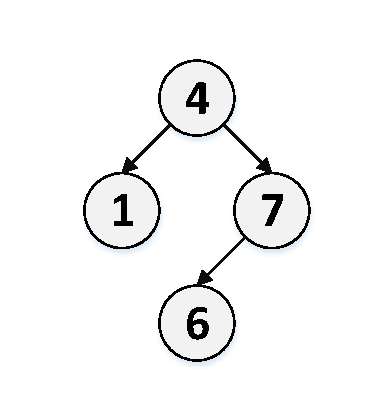
\includegraphics[width=1\columnwidth]{./graph/bst1}
        \caption{}
        \label{fig:bst1}
    \end{subfigure}
    \hfill
    \begin{subfigure}{0.32\columnwidth}
        \centering
        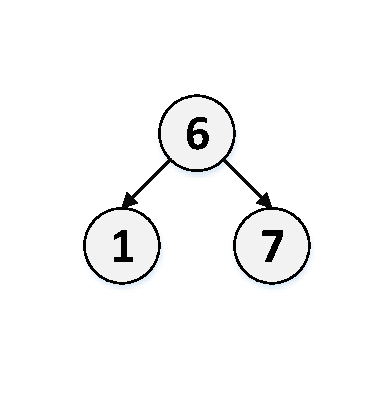
\includegraphics[width=1\columnwidth]{./graph/bst2}
        \caption{}
        \label{fig:bst2}
    \end{subfigure}
    \begin{subfigure}{0.32\columnwidth}
        \centering
        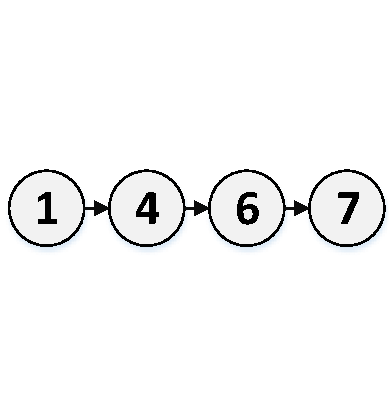
\includegraphics[width=1\columnwidth]{./graph/bst3}
        \label{fig:bst3}
        \caption{}
    \end{subfigure}
    \caption{BSTs have various layouts for the same logical ordering (a and b). The linked list (c) has deterministic layout that is independent of execution histories.}
    \label{fig:bst}
    \vspace{-0.2in}
\end{figure}

\section{Multi-dimensional Linked List}
\label{sec:mdlist}
An MDList conveniently lends support to designing high-performance lock-free \textsc{Find}, \textsc{Insert} and \textsc{Delete} operations because of its distributed and deterministic layout.
The core idea of an MDList is to partition a linked list into shorter sub-lists and rearrange them in a multi-dimensional space to facilitate search.
For brevity, we provide the definition of an MDList as below but refer readers to the authors' previous work~\cite{zhang2015lockfree} for detailed explanation on MDList intuitions and sequential algorithms.

\begin{definition}
\label{def:mdlist}
A $D$-dimensional list is a rooted tree in which each node is implicitly assigned a dimension of $d \in [0,D)$. The root node's dimension is $0$. A node of dimension $d$ has no more than $D-d$ children, and each child is assigned a unique dimension of $d' \in [d,D)$.
\end{definition}
\vspace{-0.05in}

In an ordered multi-dimensional list, we associate every node with a coordinate vector $\mathbf{k}$, and determine the order among nodes lexicographically based on $\mathbf{k}$.
A dimension $d$ node share a coordinate prefix of length $d$ with its parent.
The following requirement prescribes the exact arrangement of nodes according to their coordinates.
\vspace{-0.05in}
\theoremstyle{definition}
\begin{definition}
\label{def:mdlistsort}
    Given a non-root node of dimension $d$ with coordinate $\mathbf{k}=(k_0,...,k_{D-1})$ and its parent with coordinate $\mathbf{k'}=(k'_0,...,k'_{D-1})$ in an ordered $D$-dimensional list: $k_i = k'_i, \;\forall \;i \in [0, d) \land k_d > k'_d$.
\end{definition}
\vspace{-0.05in}

The search operation examines one coordinate at a time and locates correspondent partitions by traversing nodes that belong to each dimension. 
The search time is bounded by the dimensionality of the data structure and logarithmic search time is achieved by choosing $D$ to be a logarithm of the key range. 
To map a scalar key to a high-dimensional vector, one can choose any injective and monotonic function.
In this paper, we employ a base conversion function \textsc{KeyToCoord} as our mapping function~\cite{zhang2015lockfree}.
This function maps keys uniformly to the vector space, which optimizes the average search path length for random inputs.
For a key in range $[0,N)$, \textsc{KeyToCoord} converts it to the base-$\lceil \sqrt[D]{N}\rceil$ representation, and treats each digit as one coordinate.
For example, given key 1234, when $N=2^{32}$ and $D=8$ we have $(1234)_{10}=(4D2)_{16}$.
Thus the key 1234 will be mapped to vector (0,0,0,0,0,4,D,2).

\label{sec:cpdict}
\setlength{\columnsep}{8pt}
\begin{algorithm}[t]
    \caption{Lock-free Dictionary Data Structure}
    \label{alg:pqstructure}
    \vspace{-0.2in}
    \begin{multicols}{2}
        \begin{algorithmic}[1]
            \Class{Dictionary}
            \State \textbf{const int} $D$
            \State \textbf{const int} $N$
            \State \textbf{Node*} $head$
            \EndClass
            \Statex
            \Struct{Node}
            \State \textbf{int} $key, k[D]$
            \State \textbf{void*} $val$
            \State \textbf{Node*} $child[D]$
            \State \textbf{AdoptDesc*} $adesc$
            \EndStruct
            \Statex
            \Struct{AdoptDesc}
            \State \textbf{Node*} $curr$
            \State \textbf{int} $dp$ 
            \State \textbf{int} $dc$ 
            \EndStruct
            \Statex
        \end{algorithmic}
    \end{multicols}
    \vspace{-0.18in}
\end{algorithm}

\begin{algorithm}[t]
    \caption{Pointer Marking}
    \label{alg:pointermarking}
    \begin{algorithmic}[1]
        \State \textbf{int} $F_{adp} \gets \texttt{0x1},\;F_{del} \gets \texttt{0x2},\;F_{all} \gets F_{adp} | F_{del}$
        \Define{SetMark}{$p,\;m$} $(p\;|\;m)$
        \EndDefine
        \Define{ClearMark}{$p,\;m$} $(p\;\&\;\sim m)$
        \EndDefine
        \Define{IsMarked}{$p,\;m$} $(p\;\&\;m)$
        \EndDefine
    \end{algorithmic}
\end{algorithm}


\section{Lock-free Dictionary}
We define the structure of the concurrent dictionary and the auxiliary descriptor object in Algorithm~\ref{alg:pqstructure}.
The dimension of the dictionary is denoted by a constant integer $D$ and the range of the keys by $N$.
A node contains a key-value pair, an array $k[D]$ of integers that caches the coordinate vector to avoid repetitive computation, a descriptor for the child adoption process (detailed in Section~\ref{sec:dictins}), and an array of child pointers in which the $d$th pointer links to a dimension $d$ child node.
A descriptor~\cite{herlihy2012art} is an object that stores operation context used by helping threads to finish a delayed operation.
For a dimension $d$ node, only the indices in $[d,D)$ of its child array are valid and the rest are unused~\footnote{Since nodes of higher dimensions have less children, for a $d$ dimension node it is possible to allocate a child array of size $d$ to reduce memory consumption. In this paper, we demonstrate the use of constant size child array for simplicity.}.
The dictionary is initialized with a dummy head node, which has the minimal key 0.
We employ the pointer marking technique~\cite{harris2001pragmatic} to mark adopted child nodes as well as logically deleted nodes. 
The macros for pointer marking are defined in Algorithm~\ref{alg:pointermarking}.
$F_{adp}$ and $F_{del}$ flags are co-located with the $child$ pointers.

\begin{figure}[t]
    \centering
    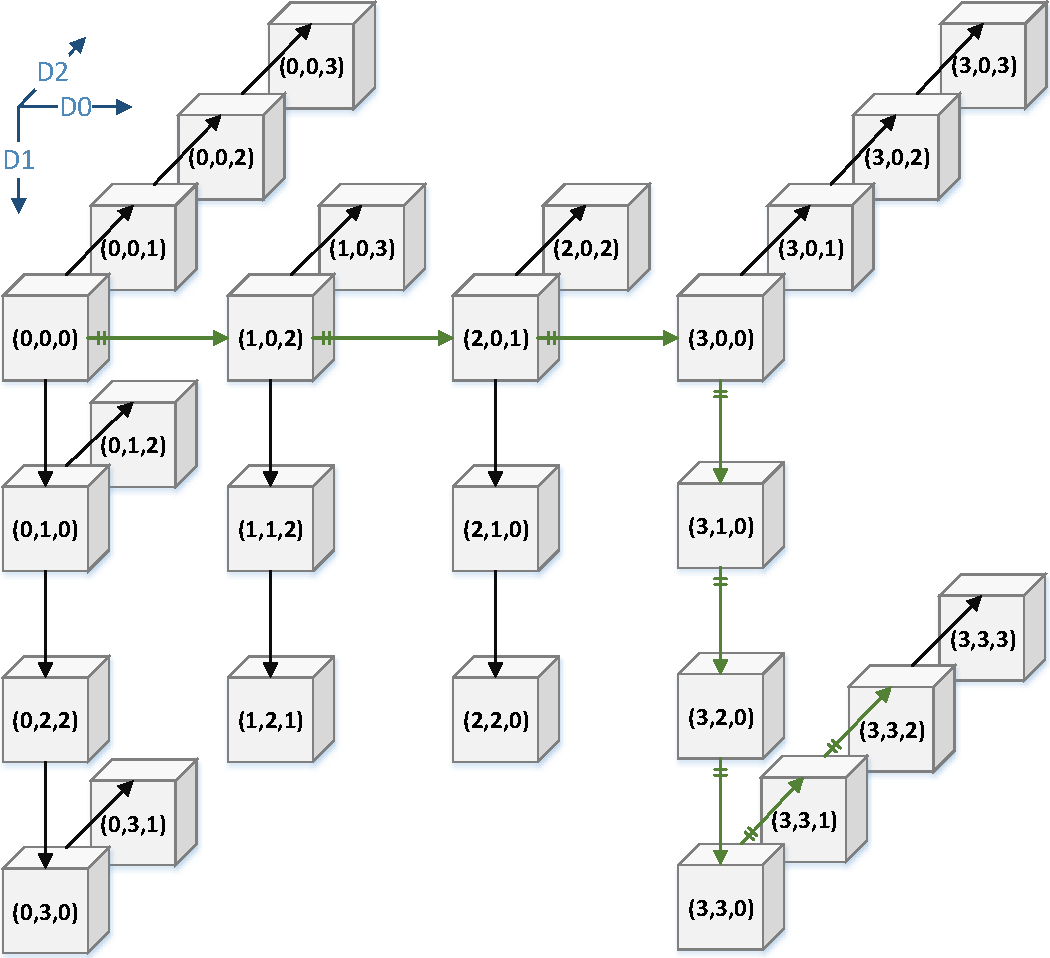
\includegraphics[width=1\columnwidth]{./graph/mdlist-3d}
    \caption{\textsc{Find} operation in a 3DList ($D=3,N=64$)}
    \label{fig:mdlist3d}
    \vspace{-0.22in}
\end{figure}

\subsection{Concurrent Find}
\label{sec:cdictfind}
We illustrate the \textsc{Find} operation on an example 3DList in Figure~\ref{fig:mdlist3d}.
To locate the node with key 62 (coordinates (3,3,2)), the \textsc{Find} operation traverse 3 sub-lists following the path highlighted by the green arrows. 
The worst-case time complexity of the search algorithm is $\mathcal{O}(D \cdot M)$ where $M$ is the maximum number of nodes in each dimension.
If we use previously described \textsc{KeyToCoord} to uniformly map the keys into the $D$-dimensional vectors, $M$ is bounded by $\sqrt[D]{N}$.
This gives $\mathcal{O}(D \cdot \sqrt[D]{N})$, which is equivalent to $\mathcal{O}(\log{N})$, if we choose $D \propto \log{N}$ (Note that $\sqrt[\log{N}]{N}=2$).

We list the concurrent \textsc{Find} function in Algorithm~\ref{alg:find}.
The search begins from the head (line~\algref{alg:find}{l:findfromhead}\footnote{We use indexing notion $[a:b]$ to address elements within the range of $[a, b)$.}).
It then invokes \textsc{LocatePred} listed in Algorithm~\ref{alg:locatepred} to perform the predecessor query.
For clarity of presentation, we use the notion of \textbf{inline} functions, which have implicit access to the caller's local variables without explicit argument passing.
The \textsc{LocatePred} function is an extension of the sequential MDList search function~\cite{zhang2015lockfree}.
Given a coordinate vector $k$, it tries to determine its immediate parent $pred$ and child $curr$.
In the case that the node with the target coordinates already exists, $curr$ points to the node itself.
Together with the dimension variables $dp$ and $dc$, they amount to the context for inserting or deleting nodes.
On line~\algref{alg:locatepred}{l:help}, prior to reading $curr$'s child \textsc{LocatePred} helps finish any child adoption tasks in order to acquire the up-to-date values.
Since a child adoption process updates the children indexed from $dp$ to $dc$, the function must help $curr$ node if it intends to read the child node in this range (line~\algref{alg:locatepred}{l:helprange}).
The helping task does not alter already traversed nodes, so the search process can continue without restart.

\begin{algorithm}[t]
    \caption{Concurrent Find}
    \label{alg:find}
    \begin{algorithmic}[1]
        \Function{Find}{$\textbf{int}\;key$}
        \State \textbf{Node*} $curr,\;pred$ 
        \State \textbf{int} $dp,\;dc$ 
        \State $pred \gets \NIL,\;curr \gets head,\;dp \gets 0,\;dc \gets 0$ \label{l:findfromhead}
        \State \Call{LocatePred}{$\textsc{KeyToCoord}(key)$} 
        \If{$dc = D$} \label{l:checkfind}
        \State \Return $curr.val$
        \Else
        \State \Return \NIL
        \EndIf
        \EndFunction
    \end{algorithmic}
\end{algorithm}
%\vspace{-14pt}
\begin{algorithm}[t]
    \caption{Predecessor Query}
    \label{alg:locatepred}
    \begin{algorithmic}[1]
        \Inline{LocatePred}{\textbf{int} $k[\;]$}
        \While {$dc < D$} \label{l:locatewhile}
        \While {$curr\neq\NIL \AND k[dc] > curr.k[dc]$} \label{l:predcheck1}
        \State $pred \gets curr,\:dp \gets dc$ \label{l:dp}
        \State $ad \gets curr.adesc$ 
        \If{$ad \neq \NIL \AND dp \in [ad.dp,\;ad.dc]$} \label{l:helprange}
        \State \Call{FinishInserting}{$curr,\;ad$} \label{l:help}
        \EndIf
        \State $curr\gets\textsc{ClearMark}(curr.child[dc],F_{all})$ \label{l:readcurr}
        \EndWhile
        \If {$curr=\NIL \OR k[dc] < curr.k[dc]$} \label{l:predcheck2}
        \State \BREAK
        \Else
        \State $dc \gets dc+1$ \label{l:dc}
        \EndIf
        \EndWhile
        \EndInline
    \end{algorithmic}
\end{algorithm}
%\vspace{-14pt}

\subsection{Concurrent Insert}
\label{sec:dictins}
The lock-free \textsc{Insert} operation is derived from the sequential MDList algorithm~\cite{zhang2015lockfree}, in which each insertion takes one or two steps and updates no more than two consecutive nodes.
Figure~\ref{fig:mdlist3dins} illustrates the insertion of key 32 (coordinates (2,0,0)).
In the first step, we update the predecessor node: the new node is spliced with its predecessor on dimension 0 (as marked the by green arrows), and the old child of the predecessor becomes a dimension 2 child of the new node.
In the second step, we update the successor node if its dimensionality has changed during the first step.
In this case, the new node adopts child nodes of its successor between dimension $[0,2)$ (as marked by the red arrows).
We guarantee lock-free progress in the node splicing step by atomically updating predecessor's child pointer using CAS~\cite{harris2001pragmatic}. 
To provide for lock-free progress in the child adoption step, we need to announce the operation globally using descriptor objects~\cite{herlihy2012art}. 
This allows the interrupting threads to help finish the operation in case the insertion thread is preempted.

\begin{figure}[t]
    \centering
    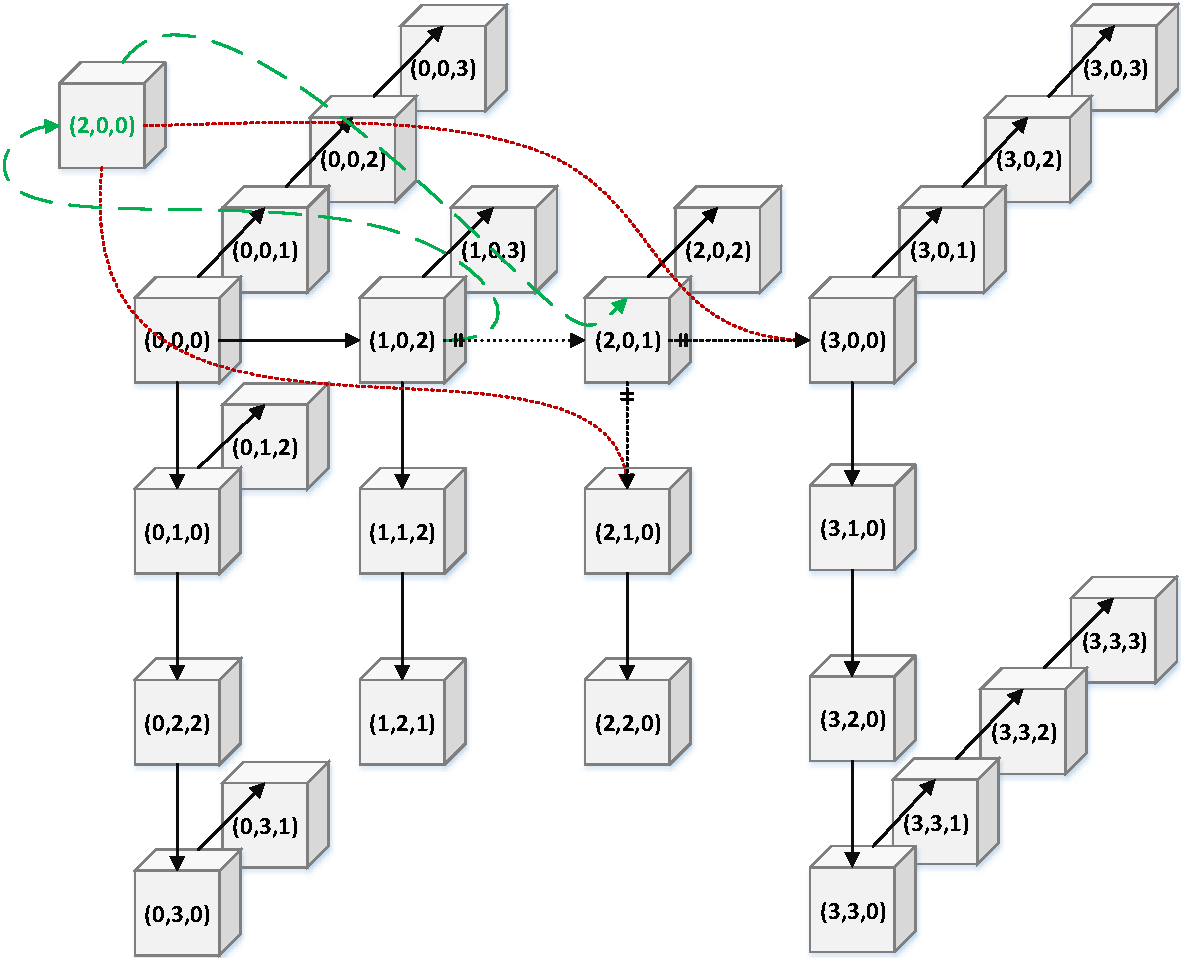
\includegraphics[width=1\columnwidth]{./graph/mdlist-3d-ins}
    \caption{\textsc{Insert} operation in a 3DList ($D=3,N=64$)}
    \label{fig:mdlist3dins}
    \vspace{-0.22in}
\end{figure}

We list the concurrent \textsc{Insert} function in Algorithm~\ref{alg:insert}.
After locating the target position (line~\algref{alg:insert}{l:locpre1}), the function updates the child pointer of the predecessor node (line~\algref{alg:insert}{l:link}).
The dimension of the node being inserted is kept in $dp$ and the dimension of the child in $dc$ (line~\algref{alg:locatepred}{l:dp} and~\algref{alg:locatepred}{l:dc}).
The new node should be inserted at the dimension $dp$ child of the $pred$ node, while a non-empty $curr$ node will become the dimension $dc$ child of the new node.
%The conditional check on line~\algref{alg:insert}{l:dupnode} is true when a node with the same coordinates already exists, thus the insertion terminates.
The code between lines~\algref{alg:insert}{l:beginhelp} and~\algref{alg:insert}{l:endhelp} reads the $adesc$ fields from $curr$ and tests if helping is needed.
Like in \textsc{LocatePred}, the insertion need to help $curr$ node if it is going to adopt children from $curr$ node.

\begin{algorithm}[t]
    \caption{Concurrent Insert}
    \label{alg:insert}
    \begin{algorithmic}[1]
        \Function{Insert}{$\textbf{int}\;key,\;\textbf{void*}\;val$}
        \State \textbf{Node*} $node$ 
        \Comment the new node
        \State \textbf{Node*} $pred,\;curr$ 
        \Comment new node's parent and child
        \State \textbf{int} $dp,\;dc$ 
        \Comment dimension of node in pred and curr 
        \State \textbf{AdoptDesc*} $ad$
        \Comment descriptor for child adoption task
        \State $node \gets \text{\textbf{new Node}}$
        \State $node.key \gets key,\;node.val \gets val$
        \State $node.k[0:D] \gets \text{\textsc{KeyToCoord}}(key)[0:D]$
        \State $node.child[0:D] \gets \NIL$
        \While{\TRUE}
        \State $pred \gets \NIL,\;curr \gets head,\;dp \gets 0,\;dc \gets 0$ \label{l:insfromhead}
        \State \Call{LocatePred}{$node.k$} \label{l:locpre1}
        \State $ad \gets curr\ne\NIL\;?\;curr.adesc\;:\;\NIL$ \label{l:beginhelp}
        \If{$ad \ne \NIL \AND dp \ne dc$}
        \State \Call{FinishInserting}{$curr,\;ad$} \label{l:endhelp}
        \EndIf
        \If {$\textsc{IsMarked}(pred.child[dp],F_{del})$} \label{l:checkdel}
        \State $curr \gets \textsc{SetMark}(curr,F_{del})$
        \If {$dc = D - 1$} \label{l:checkinfrontdel} 
        \State $dc \gets D$ \label{l:setdel}
        \EndIf
        \EndIf
        \State \Call{FillNewNode}{ } \label{l:callfillnode}
        \If {$\text{\textsc{CAS}}(\&pred.child[dp],\;curr,\;node)$} \label{l:link}
        \If {$ad \ne \NIL$}
        \State \Call{FinishInserting}{$node,\;ad$}
        \EndIf
        \State \BREAK \label{l:insret}
        \EndIf
        \EndWhile
        \EndFunction
        \State
        \Inline{FillNewNode}{ } \label{l:fillnode}
        \State $ad \gets \NIL$ \label{l:beginfill}
        \If {$dp \ne dc$}
        \State $ad \gets \text{\textbf{new AdoptDesc}}$
        \State $ad.curr \gets curr,\;ad.dp \gets dp,\;ad.dc \gets dc$ \label{l:filldesc}
        \EndIf
        \State $node.child[0:dp] \gets F_{adp}$ \label{l:initadp}
        \State $node.child[dp:D] \gets \NIL$ 
        \If {$dc < D$}
        \State $node.child[dc] \gets curr$ \label{l:physicaldel}
        \EndIf
        \State $node.adesc \gets ad$ \label{l:endfill} 
        \EndInline
    \end{algorithmic}
\end{algorithm}
\begin{algorithm}[t]
    \caption{Child Adoption}
    \label{alg:adoption}
    \begin{algorithmic}[1]
        \Function{FinishInserting}{$\textbf{Node*}\:n,\;\textbf{AdoptDesc*}\:ad$}
        \State \textbf{Node*} $child,\;curr \gets ad.curr$ 
        \State \textbf{int} $dp \gets ad.dp,\;dc \gets ad.dc$
        \For {$i \in [dp, dc)$} \label{l:adoptionfor}
        \State $child \gets \textsc{FetchAndOr}(\&curr.child[i],\;F_{adp})$ \label{l:setadp} 
        \State $child \gets \textsc{ClearMark}(child,\;F_{adp})$
        \If{$n.child[i] = \NIL$} \label{l:checkadopt}
        \State $\text{\textsc{CAS}}(\&n.child[i],\;\NIL,\;child)$ \label{l:adopt}
        \EndIf
        \EndFor
        \State $\text{\textsc{CAS}}(\&n.adesc,\;ad,\;\NIL)$
        \EndFunction
    \end{algorithmic}
\end{algorithm}


Prior to atomically updating the link to the new node, we fill the remaining fields of the new node (line~\algref{alg:insert}{l:beginfill} and~\algref{alg:insert}{l:endfill}).
If the new node needs to adopt children from $curr$ node, we use an adopt descriptor to store the necessary context (line~\algref{alg:insert}{l:filldesc}).
The pointers within the range $[0, dp)$ of the new node's child array are marked with $F_{adp}$.
This effectively invalidates these positions for future insertions.
The pointers within the range $[dp, D]$ are set to \textsc{NIL} meaning they are available for attaching child nodes.
$curr$ node is conditionally linked to the new node on line~\algref{alg:insert}{l:physicaldel}.
$dc$ can be set to $D$ on either line~\algref{alg:insert}{l:setdel} or line~\algref{alg:locatepred}{l:dc}. 
In the first case, $curr$ must be logically deleted, and the new node is immediately in front of $curr$.
By not linking it with the new node, we effectively discard $curr$.
In the second case, the new node has the same key as $curr$ and we essentially update the associated value by replacing $curr$ with the new node. 
On line~\algref{alg:insert}{l:link}, the single-word CAS atomic synchronization primitive is used to update the $pred$'s child pointer.
The CAS would fail under three circumstances: 1) the desired child slot has been updated by another competing insertion; 2) the desired child slot has been invalidated by a child adoption process; and 3) the desired child slot has been marked for logical deletion.
If any of the above cases is true, the loop restarts.
Otherwise, the insertion proceeds to finish its own child adoption process.

The \textsc{FinishInserting} function in Algorithm~\ref{alg:adoption} performs child adoption on a given node $n$ with the descriptor $ad$.
This is a helping procedure that must correctly handle duplicate and simultaneous executions.
The function first reads the adoption context from the descriptor into its local variables.
It then transfers $curr$ node's children within the range of $[dp, dc)$ to $n$.
Before a child pointer can be copied, we must safeguard it so that it cannot be changed while the copy is in progress.
This is done by setting the $F_{adp}$ flag in the child pointers (line~\algref{alg:adoption}{l:setadp}).
Once the flag is set, the function proceeds to copy the pointer to $n$ (line~\algref{alg:adoption}{l:adopt}). 
%This latter is done only if the corresponding child of $n$ equals \textsc{NIL} (line~\algref{alg:adoption}{l:checkadopt}). 
Finally, the descriptor field in $n$ is cleared to designate the operation's completion.

\begin{algorithm}[t]
    \caption{Concurrent Delete}
    \label{alg:delete}
    \begin{algorithmic}[1]
        \Function{Delete}{$\textbf{int}\;key$}
        \State \textbf{Node*} $curr,\;pred,\;child,\;marked$ 
        \State \textbf{int} $dp,\;dc$ 
        \While{\TRUE}
        \State $pred \gets \NIL,\;curr \gets head,\;dp \gets 0,\;dc \gets 0$ \label{l:delfromhead}
        \State \Call{LocatePred}{$\textsc{KeyToCoord}(key)$} \label{l:locpredel}
        \If{$dc \ne D$} \label{l:checkexist}
        \State \Return \NIL \label{l:term1}
        \EndIf
        \State $marked \gets \textsc{SetMark}(curr,\;F_{del})$
        \State $child \gets \textsc{CAS}_{val}(\&pred.child[dp],\;curr,\;marked)$ \label{l:markdel}
        \If {$\textsc{ClearMark}(child,\;F_{del}|F_{adp}) = curr$} \label{l:cond1}
        \If {$!\textsc{IsMarked}(child,\;F_{del}|F_{adp})$} \label{l:cond2}
        \State \Return $curr.val$
        \ElsIf{$\textsc{IsMarked}(child,\;F_{del})$} \label{l:cond3}
        \State \Return \NIL
        \EndIf
        \EndIf
        \EndWhile
        \EndFunction
    \end{algorithmic}
\end{algorithm}


\subsection{Concurrent Delete}
\label{sec:cpqueuedel}
The sequential \textsc{Delete} and \textsc{Insert} operations on an MDList~\cite{zhang2015lockfree} works reciprocally: the former may promote a node to a lower dimension while the latter may demote a node to a higher dimension.
This works well for sequential algorithms, but in concurrent execution where threads help each other, bidirectional change of nodes' dimension incurs contention and synchronization issues.
Consider a node $n$ with an active child adoption descriptor (i.e., $n.adesc\neq\NIL$).
When concurrency level is high, several threads may read this descriptor and proceed to help finish the adoption by marking some children on node $n.adesc.curr$ as invalid.
One of them will eventually succeeds in finish the helping (as observed by setting $n.adesc\gets \NIL$), but we have no way to know \emph{if all threads have finished the helping}.
If a \textsc{Delete} operation promotes the node $n.adesc.curr$ by re-enabling the invalid child pointers, an unfinished helping process may erroneously disable them again.
Additional synchronization is required to prevent threads from interfering with each other when they perform helping task on the same node.
We found the simplest solution is to \emph{keep dimensionality change unidirectional}.

Our lock-free \textsc{Delete} operation is thus asymmetrical in the sense that it dose not remove any node from the data structure nor alter the nodes' dimensionality.
It only marks a node for logical deletion~\cite{harris2001pragmatic}, and leaves the execution of physical removal to subsequent \textsc{Insert} operations.
When a new node ($n_n$) is inserted immediately before a logically deleted node ($n_d$), $n_n$ expunge $n_d$ from the data structure by skipping $n_n$ and linking directly into all of the child nodes of $n_d$.
Since the physical deletion is embedded in the insertion operation, we reduce the interaction between insertion and deletion operations to a minimal and achieved an overall simple design of lock-free dictionary.
%Logical deletion speeds up deletion operation by performing physically deletion in batch or at a later stage when the memory accesses are less congested.
%Our concurrent \textsc{Delete} function as shown in Algorithm~\ref{alg:delete} is lightweight because we choose to embed the physical deletion in the \textsc{Insert} function.
This may sound counterintuitive, but the list-like partition strategy of MDList allow us to efficiently discard nodes by simply skipping links. 
Since a logically deleted node only gets purged when an insertion take place immediately in front of it, there will be a number of zombie nodes.
We thus trade memory consumption for scalability.
%On the other hand, there is less chance that physical deletions can interfere with concurrent insertion.
We thus trade memory consumption for scalability.

In Algorithm~\ref{alg:delete}, the concurrent \textsc{Delete} operation traverses the dictionary starting from the head looking for target node.
It shares the same CAS-based loop as the \textsc{Insert} function.
The process terminates on line~\algref{alg:delete}{l:term1} if it fails to find the target node.
Otherwise, it marks the target node for logical deletion using CAS~\algref{alg:delete}{l:markdel}.
A node is considered logically deleted once the pointer in its parent's child array is marked with $F_{del}$.
The $\text{CAS}_{val}$ returns the value store on the address before the update.
It is considered successful if the return value $child$ is equal to the expected value $curr$, which is detected by the conditional statement on line~\algref{alg:delete}{l:cond1} and~\algref{alg:delete}{l:cond2}.
Otherwise, the function checks if the target node has already been marked for deletion by examine the $F_{del}$ flag on $child$ (line~\algref{alg:delete}{l:cond3}).
If so, the function returns.
Finally, the child pointer in $pred$ must have been updated by concurrent insertions, \textsc{Delete} would start anew from the head.

\section{Correctness}
\label{sec:correctness}
In this section, we sketch a proof of the main correctness property of the presented dictionary algorithm, which is linearizability~\cite{herlihy1990linearizability}. 
A concurrent object is linearizable if all of its operations appear to take effect instantaneously at some point after the operations start and before they end.
We begin by defining the \emph{abstract state} of a sequential dictionary and then show how to map the internal state of our concrete dictionary object to the abstract state.
We denote the abstract state of a sequential dictionary to be a totally ordered set $P$.
Equation~\ref{eq:insert} specifies that an \textsc{Insert} operation grows the set if the key being inserted does not exist.
Equation~\ref{eq:delete1} specifies that a \textsc{Delete} operation shrinks a non-empty set by removing the key-value pair with the specific key.
\vspace{-0.06in}
\begin{equation} \label{eq:insert}
    \textsc{Insert}(\langle k,v \rangle)= \begin{cases}
        P \cup \{\langle k,v\rangle\} & \forall \langle k',v'\rangle \in P\;,\;k' \neq k\\
        P & \exists \langle k',v' \rangle \in P : k'=k
    \end{cases}
\end{equation}

\begin{gather}
    \label{eq:delete1}
    \textsc{Delete}(k)= \begin{cases}
        P \setminus \{\langle k,v \rangle\} & \langle k,v\rangle \in P\\
        P & \langle k,v\rangle \notin P
    \end{cases}
\end{gather}

\subsection{Invariants}
Now we consider the concurrent dictionary object. 
By a \emph{node}, we refer to an object of type \textbf{Node} that has been allocated and successfully linked to an existing node (line~\algref{alg:insert}{l:link}). 
We denote the set of nodes that are reachable from $head$ by $L$. 
The following invariants are satisfied by the concrete dictionary object at all times. 
Invariant~\ref{inv:adpflag} states that if a node has no pending child adoption task, its dimension $d$ child must have $d$ invalid child slots leaving $D-d$ valid ones.

\begin{invariant} \label{inv:adpflag}
$\forall n,n' \in L,\textsc{ClearMark}(n.child[d],F_{adp}\linebreak|F_{del})=n'\;\land\;n.adesc=\NIL \implies \forall i \in [0,d), \textsc{IsMarked}(\linebreak n'.child$ $[i],F_{adp})=\TRUE$
\end{invariant}
\begin{proof}
    By observing the statements at line~\algref{alg:insert}{l:initadp} and~\algref{alg:adoption}{l:setadp} we see that the $F_{adp}$ flags are properly initialized before linking a new node to its predecessor and updated properly whenever a child is adopted.
\end{proof}

Invariant~\ref{inv:reachability} states that any node in $L$ can be reach by following a series child pointers with non-decreasing dimensionality.

\begin{invariant} \label{inv:reachability}
    $\forall n \in L, \exists p=\{d_0,d_1,...,d_m\} : d_0\le d_1 \le ... \le d_m\;\land\;head.child[d_0].child[d_1]...child.[d_m]=n$
\end{invariant}
\begin{proof}
    At the start, the structure contains a dummy $head$ node and the invariant holds trivially. 
    Any new node is initially placed at a position reachable from $head$ because the node traversed by \textsc{LocatePred} (Algorithm~\ref{alg:locatepred}) form a consecutive path $p'$.
    Note the condition checks in (line~\algref{alg:locatepred}{l:predcheck1} and~\algref{alg:locatepred}{l:predcheck2}), we have $i<j \implies d_i \leq d_j \;\forall d_i,d_j \in p'$.
    Though subsequent insertions may alter the path, they do not unlink nodes from the data structure.
    The claim follows by noting that an insertion either adds a new node to $p'$ or replaces an existing node in $p'$. 
    %Future insertions either replace a node in $p$ or add a new node.
%If $dp = dc$, add new link, if $dp < dc if dp < d_1 < dc d_1$ is adopted,link replace, if $d_1 > dc$, add new link. 
\end{proof}

\begin{lemma} \label{lmm:mdlist}
    At any time, nodes in $L$, including those marked for logical deletion, form an MDList that complies with Definition~\ref{def:mdlist}.
\end{lemma}
\begin{proof}
    Invariant~\ref{inv:adpflag} shows that for any node $n$ with dimension $d$, only children with dimension greater or equal to $d$ is accessible, thus the dimension of a node is always no greater than the dimensions of its children.
    Follow Invariant~\ref{inv:reachability}, logically deleted key-value pairs still occupy valid nodes in the structure before they are physically removed.
\end{proof}

%\begin{lemma}
%LocatePred always find earlies insertion position, never overshoot even when child slot is invalidated
%Because a unique path exist if a node is in the set
%So if a node is in the set, LocatePred will be able to reach it and dc = D, this guarantees that no duplicate keys will be inserted.
%\end{lemma}
%\begin{proof}
    %Follow Invariant~\ref{inv:link}, and above lemma. 
    %A node in th set can be reached through a serial of child[i] pointers where i is increasing
    %define the sequence of pointers as unique search path
%\end{proof}

We now show that the nodes \emph{without} deletion marks form a well-ordered set that is equivalent to $P$.
Invariant~\ref{inv:order} states that the ordering property described by Definition~\ref{def:mdlistsort} is kept at all times.

\begin{invariant} \label{inv:order}
    $\forall n,n' \in L, n.child[d]=n' \implies n.key < n'.key$ $\land\;\forall i \in [0, d)\; n.k[i] = n'.k[i] \land n.k[d]<n'.k[d]$
\end{invariant}
\begin{proof}
    Initially the invariants trivially holds.
    The linkage among nodes is only changed by insertion, and child adoption.
    Insert preserves the invariants because the condition checks on line~\algref{alg:insert}{l:predcheck1} and~\algref{alg:insert}{l:predcheck2} guarantee that $\forall i \in [0, dp)\; pred.k[i] = node.k[i] \land pred.k[dp]<node.k[dp]$.
    Child adoption preserves the invariant because $\forall i \in [dp, dc)\; node.k[i] = curr.k[i] < curr.child[i].k[i]$.
%A node's dimensionality only increases, never decreases.
%Note invariant $dc \ge dp$
\end{proof}

\begin{lemma} \label{lmm:logical}
    Logically deleted nodes appear transparent to traversing operations.
\end{lemma}
\begin{proof}
    Note that a pointer to logically deleted nodes is marked by flag $F_{del}$, which renders the key-value pair stored in that node obsolete.
    However, the node's location withing the data structure is still consistent with its embed coordinates, making it a valid routing node.
    The traversing operation treat logically deleted nodes transparently by explicitly clearing the pointer markings on line~\algref{alg:locatepred}{l:readcurr}. 
\end{proof}

%\begin{lemma} \label{lmm:adoption}
    %Child adoption appears transparent to traversing operations
%\end{lemma}
%\begin{proof}
    %The adoption descriptor object is set only once for each node (line~\algref{alg:insert}{l:endfill}), and is cleared after completion.
    %All accesses to child slots are preclude by FinishInserting, forcing child adoption ensuring consistency.
    %Finishing the adesc before accessing nodes with adesc set 
%\end{proof}

Let us define the set of logically deleted nodes by $S=\{n|n'\in L \land n'.child[d] = \textsc{SetMark}(n, F_{del})\}$.
Following Lemma~\ref{lmm:mdlist} and~\ref{lmm:logical}, the abstract state can then be defined as $P \equiv L \setminus S$.

\subsection{Linearizability}
We now sketch a proof that our algorithm is a linearizable dictionary implementation that complies with the abstract semantics by identifying \emph{linearization points} for each operation.
The concurrent operation can be viewed as it occurred atomically at its linearization point in the execution history.
Additionally, we use the notion of decision points and state-read points to facilitate our reasoning~\cite{sundell2004scalable}. 
The decision point of an operation is define as the atomic statement that finitely decides the result of an operation, i.e. independent of the result of any subsequent instruction after that point.
A state-read point is define as the atomic statement where the state of the dictionary, which determines the outcome of the decision point, is read.

\begin{theorem}
    A $\textsc{Find}(k)$ operation takes effect atomically at one statement.
\end{theorem}
\begin{proof}
    A find operation may return $v$ if $\langle k,v \rangle \in P$, or $\NIL$ otherwise.  
    The decision point for the first case is when the \texttt{while} loop terminates on line~\algref{alg:locatepred}{l:locatewhile}.
    The node with $k$ must exist in $P$ because the coordinates up to dimension $D$ have been exhaustively examined.
    The state-read point is line~\algref{alg:locatepred}{l:readcurr} when $curr$ is read from child pointers.
    The subsequent execution branches to line~\algref{alg:locatepred}{l:dc} after comparing $curr.k$ with $k$.
    As the coordinate field $k$ cannot be changed after initialization, the state of the dictionary immediate before passing the state-read point must have been $\langle k,v \rangle \in P$.
    The decision point for the second case is when the condition check on line~\algref{alg:locatepred}{l:predcheck2} fails.
    The state-read point is when the value of $curr$ is read on line~\algref{alg:locatepred}{l:readcurr}.
    For both case, the linearization point is the state-read point on line~\algref{alg:locatepred}{l:readcurr}
\end{proof}

\begin{theorem}
    An $\textsc{Insert}(\langle k,v\rangle)$ operation takes effect atomically at one statement.
\end{theorem}
\begin{proof}
    An \textsc{Insert} operation returns on line~\algref{alg:insert}{l:insret}; given a legal key it must succeed by either adding a new node or replacing an existing node.
    The decision point for both cases to take effect is when the CAS operation on line~\algref{alg:insert}{l:link} succeeds.
    The remaining atomic primitives in the child adoption process will be executed at least once and successfully complete through the use of helping mechanism.
    Equation~\ref{eq:insert} holds for the first case because $L=L\cup \langle k,v \rangle$.
    It holds for the second case because $L=L\cup \langle k,v \rangle \setminus \langle k,v' \rangle$.
\end{proof}

\begin{theorem}
    A $\textsc{Delete}(k)$ operation takes effect atomically at one statement.
\end{theorem}
\begin{proof}
    If $\langle k,v \rangle \in P$, a successful $\textsc{Delete}(k)$ operation updates the abstract state by growing $S$.
    The decision point for it to take effect is when the CAS operation on line~\algref{alg:delete}{l:markdel} successfully marks a node for deletion.
    Equations~\ref{eq:delete1} holds because $S' = S \cup \langle k,v \rangle \implies P' = P \setminus \{\langle k,v \rangle$\}.
    The decision points for a $\textsc{Delete}(k)$ operation to fail are on line~\algref{alg:delete}{l:checkexist} when it cannot find the node with the target key, and on line~\algref{alg:delete}{l:cond3} when the target node has been logically deleted by a competing deletion operation.
    The state-read point for the former is on line~\algref{alg:locatepred}{l:readcurr}, which causes \textsc{LocatePred} to abort before reaching the highest dimension.
    The state-read point for the latter is on line~\algref{alg:delete}{l:markdel}, where $child$ is read.
    The linearization points for failed deletions are either of the state-read points.
    In these cases, Equations~\ref{eq:delete1} holds because $S' = S \implies P' = P$.
\end{proof}

\subsection{Lock Freedom}
Our algorithm is lock-free because it guarantee that for every possibly execution scenario, at least one thread makes progress.
We prove this by examining unbounded loops in all possible execution paths, which can delay the termination of the operations.
\begin{lemma} \label{lmm:finitestep}
    \textsc{FinishInserting} (Algorithm~\ref{alg:adoption}) and \textsc{LocatePred} (Algorithm~\ref{alg:locatepred}) complete in finite steps.
\end{lemma}
\begin{proof}
    We observe that there is no unbounded loop in Algorithm~\ref{alg:adoption}.
    The \texttt{for} loop on line~\algref{alg:adoption}{l:adoptionfor} is bounded by the dimensionality of data structure $D$, which in practice is a small number.
    For \textsc{LocatePred}, the \texttt{while} loop (line~\algref{alg:locatepred}{l:locatewhile}) is also bounded by $D$.
    The inner unbounded \texttt{while} loop (~\algref{alg:locatepred}{l:predcheck1}) ends after at most $\sqrt[D]{N}$ retries, which is the maximum number of nodes in each dimension.
    The maximum number of nodes to be examined by \textsc{LocatedPred} is thus $D \cdot \sqrt[D]{N}$.
\end{proof}

\begin{theorem}
    \textsc{Find} operations are wait-free.
\end{theorem}
\begin{proof}
    The \textsc{Find} operations invoke \textsc{LocatePred} and does not contain additional loops. 
    The theorem holds by following Lemma~\ref{lmm:finitestep} 
\end{proof}

\begin{theorem}
    \textsc{Insert} and \textsc{DeleteMin} operations are lock-free.
\end{theorem}
\begin{proof}
    Note that all shared variables are concurrently modified by CAS operations, and the CAS-based unbounded loops (line~\algref{alg:insert}{l:link}, and~\algref{alg:delete}{l:markdel} only retry when a CAS operation fails.
    This means that for any subsequent retry, there must be one CAS that succeeded, which caused the termination of the loop.
    All reads of child pointer are preceded by \textsc{FinishInserting}, which completes child adoption in finite steps to ensure consistency.
    Furthermore, our implementation does not contain cyclic dependencies between CAS-based loops, which means that the corresponding operation will progress.
\end{proof}

\begin{figure*}[t]
    \begin{subfigure}{0.32\textwidth}
        \centering
        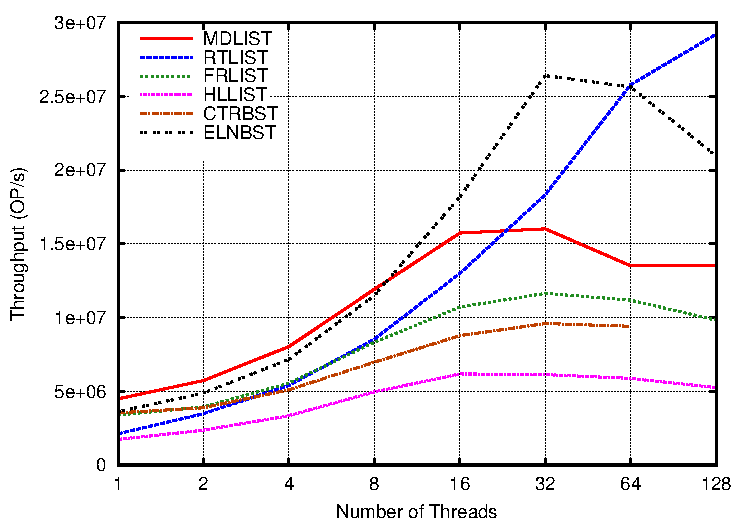
\includegraphics[width=1\columnwidth]{./data/amd50ins1Kkey}
        \caption{1K keys}
        \label{fig:1k50ins}
    \end{subfigure}
    \hfill
    \begin{subfigure}{0.32\textwidth}
        \centering
        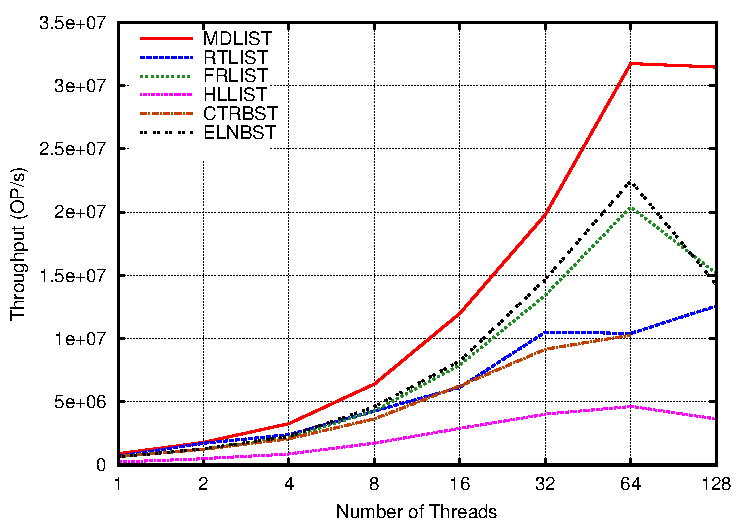
\includegraphics[width=1\columnwidth]{./data/amd50ins1Mkey}
        \caption{1M keys}
        \label{fig:1m50ins}
    \end{subfigure}
    \hfill
    \begin{subfigure}{0.32\textwidth}
        \centering
        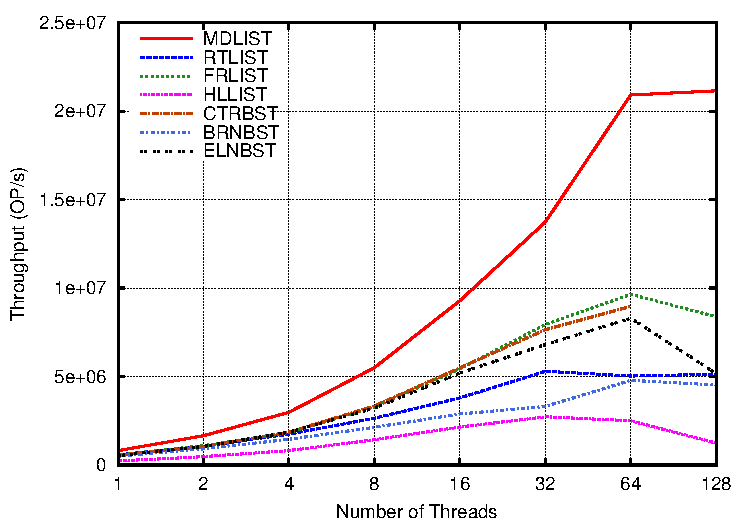
\includegraphics[width=1\columnwidth]{./data/amd50ins1Bkey}
        \caption{1G keys}
        \label{fig:1b50ins}
    \end{subfigure}
    \vspace{-0.08in}
    \caption{$50\%$ \textsc{Insert}, $50\%$ \textsc{Delete}, $0\%$ \textsc{Find} on the NUMA System}
    \label{fig:writeload}
\end{figure*}

\begin{figure*}[t]
    \begin{subfigure}{0.32\textwidth}
        \centering
        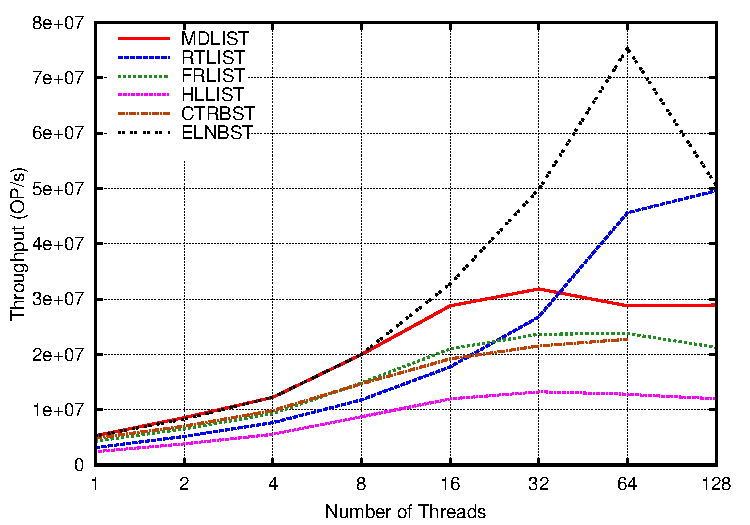
\includegraphics[width=1\columnwidth]{./data/amd20ins1Kkey}
        \caption{1K keys}
        \label{fig:1k20ins}
    \end{subfigure}
    \hfill
    \begin{subfigure}{0.32\textwidth}
        \centering
        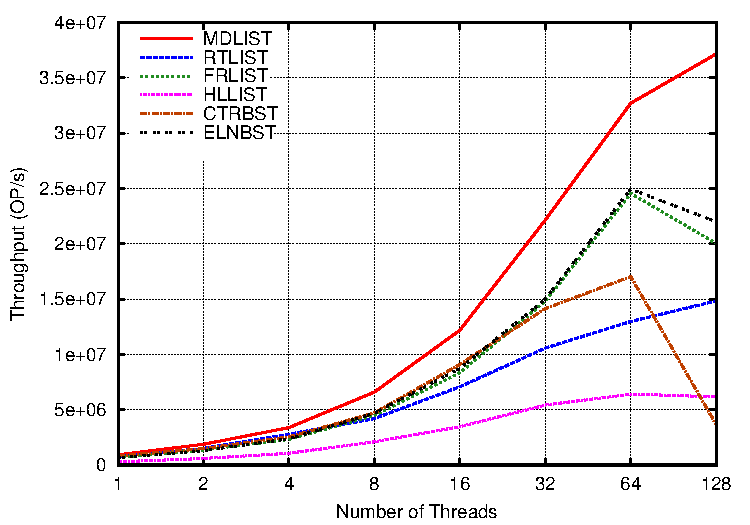
\includegraphics[width=1\columnwidth]{./data/amd20ins1Mkey}
        \caption{1M keys}
        \label{fig:1m20ins}
    \end{subfigure}
    \hfill
    \begin{subfigure}{0.32\textwidth}
        \centering
        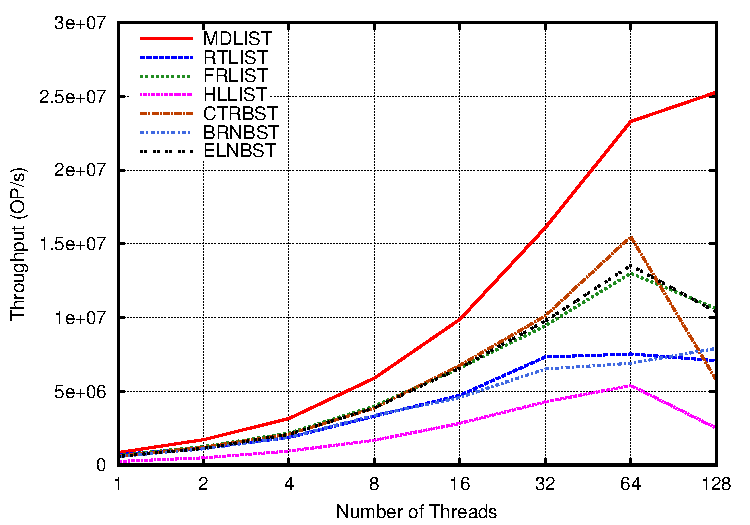
\includegraphics[width=1\columnwidth]{./data/amd20ins1Bkey}
      \caption{1G keys}
        \label{fig:1b20ins}
    \end{subfigure}
    \vspace{-0.08in}
 \caption{$20\%$ \textsc{Insert}, $10\%$ \textsc{Delete}, $70\%$ \textsc{Find} on the NUMA System}
    \label{fig:mixload}
\end{figure*}

\begin{figure*}[t]
    \begin{subfigure}{0.32\textwidth}
        \centering
        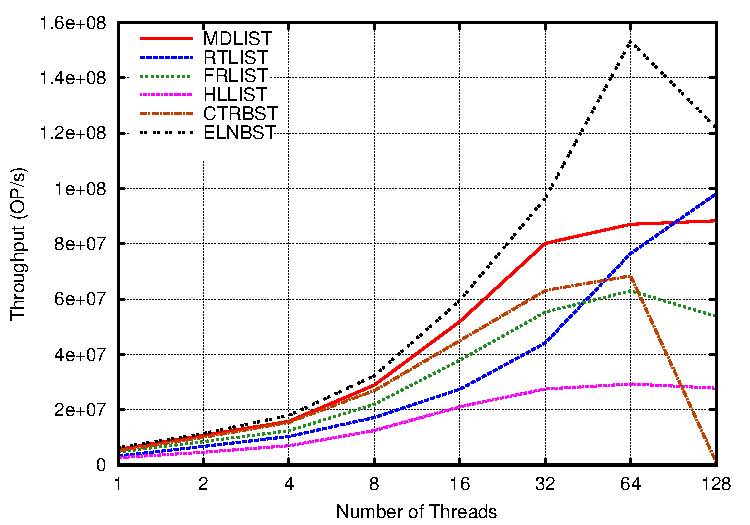
\includegraphics[width=1\columnwidth]{./data/amd9ins1Kkey}
        \caption{1K keys}
        \label{fig:1k9ins}
    \end{subfigure}
    \hfill
    \begin{subfigure}{0.32\textwidth}
        \centering
        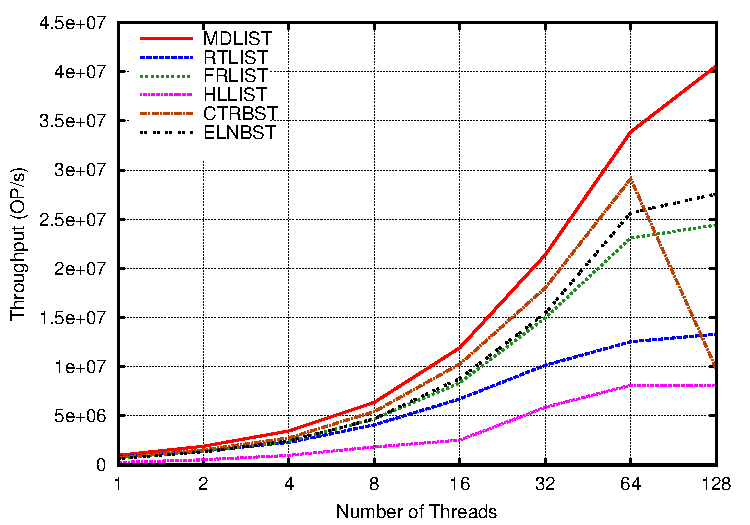
\includegraphics[width=1\columnwidth]{./data/amd9ins1Mkey}
        \caption{1M keys}
        \label{fig:1m9ins}
    \end{subfigure}
    \hfill
    \begin{subfigure}{0.32\textwidth}
        \centering
        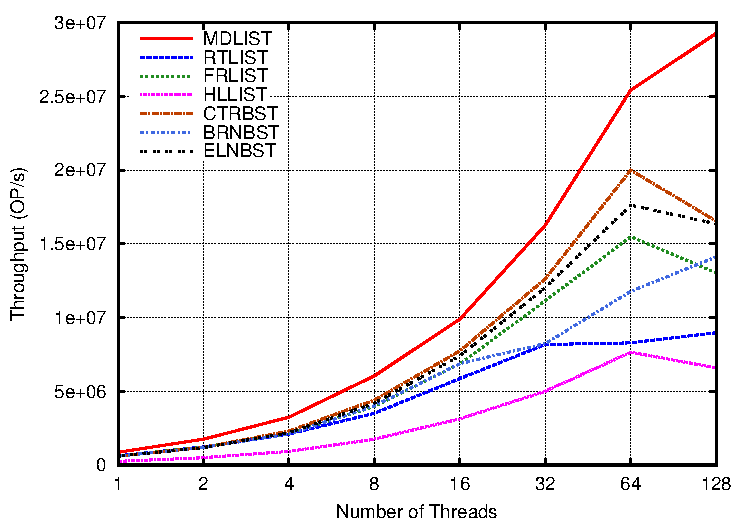
\includegraphics[width=1\columnwidth]{./data/amd9ins1Bkey}
      \caption{1G keys}
        \label{fig:1b9ins}
    \end{subfigure}
    \vspace{-0.08in}
 \caption{$9\%$ \textsc{Insert}, $1\%$ \textsc{Delete}, $90\%$ \textsc{Find} on the NUMA System}
    \label{fig:readload}
    \vspace{-0.2in}
\end{figure*}

\section{Experimental Evaluation}
\label{sec:experiment}
We compare the performance of our algorithm (MDLIST) to the following concurrent skiplists and BSTs that are available to us in C/C++ implementations.
\begin{enumerate}
    \item The rotating skiplist (RTLIST) by Dick et al.~\cite{dick2014logarithmic}. Their implementation is build upon the C port of Crain's no hot-spot skiplist~\cite{crain2013no}, which employs a background thread to maintain balance and handle physical deletions.
    \item Herlihy's lock-free skiplist~\cite{herlihy2012art} (HLLIST) with lazy deletions. The tested version is derived from Wicht's C++ implementation~\cite{wicht2012binary}.
    \item Fraser's publicly available lock-free skiplist~\cite{fraser2004practical} (FRLIST), which includes several optimizations not found in HLLIST. It is often considered as the most efficient skiplist implementation.
    \item The lock-based implementation of Bronson et al.'s relaxed AVL tree~\cite{bronson2010practical} (BRNBST) derived from Wicht's C++ implementation~\cite{wicht2012binary}.
    \item The lock-free unbalanced BST (ELNBST) based on Ellen et al's algorithm~\cite{ellen2010non}. The implementation is derived from Wicht's C++ implementation~\cite{wicht2012binary}.
    \item The Citrus tree~\cite{arbel2014concurrent} (CTRBST) by Arbel et al, which employs the novel synchronization mechanism \emph{read copy update} (RCU). RCU allows updates to produce a copy of the data they write so the read-only accesses can proceed without acquiring locks. Code is available directly from the authors.
\end{enumerate}
The original implementation of FRLIST, RTLIST and our algorithm used the epoch based garbage collection proposed by Fraser~\cite{fraser2004practical}, while BRNBST, ELNBST and HLLIST used hazard pointers~\cite{michael2004hazard}.
CTRBST, on the other hand, did not employ any memory management scheme.
For fair comparison of the algorithms themselves, we disabled memory reclamation for all approaches but use thread-caching malloc~\cite{ghemawat2009tcmalloc} as a scalable alternative to the standard library malloc.
We employ a micro-benchmark to evaluate the throughput of these approaches for uniformly distributed keys.
This canonical evaluation method~\cite{harris2001pragmatic,dick2014logarithmic,natarajan2014fast} consists of a tight loop that randomly chooses to perform an \textsc{Insert}, a \textsc{Delete} or a \textsc{Find} operation in each iteration. 
Each thread performs one million operations and we take the average from four runs.
As done in~\cite{natarajan2014fast,brown2014general} we pre-populate the data structures to half capacity to ensure consistent result.
Both the micro-benchmark and the dictionary implementations are compiled using GCC 4.7 with \texttt{O3} optimizations.
The tests are conducted on a 64-core NUMA system (4 AMD opteron CPUs with 16 cores per chip @2.1 GHz) and a 12-core SMP system (1 Intel Xeon 6-core CPU with hyper-threading @2.9GHz). 

Figures~\ref{fig:writeload}, ~\ref{fig:mixload} and~\ref{fig:readload} illustrate the algorithms' throughput on the NUMA system.
The $y$-axis represents the throughput measured by \emph{operation per second}, and the $x$-axis represents the number of threads in logarithmic scale.
Like the evaluations in~\cite{natarajan2014fast,howley2012non}, we consider three different workload distributions: a) write-dominated with $50\%$ insertion, $50\%$ deletion; b) mixed workload with $20\%$ insertion, $10\%$ deletion and $70\%$ find; c) read-dominated with $9\%$ insertion, $1\%$ deletion and $90\%$ find.
We also consider three ranges of keys, 1000 (1K), 1 million (1M) and 1 billion (1G). 
The size of key space affects the height of search trees, but it does not affect the tower height of a skiplist nor the dimension of an MDList as those are chosen by users prior to execution.
\begin{figure*}[t]
    \begin{subfigure}{0.32\textwidth}
        \centering
        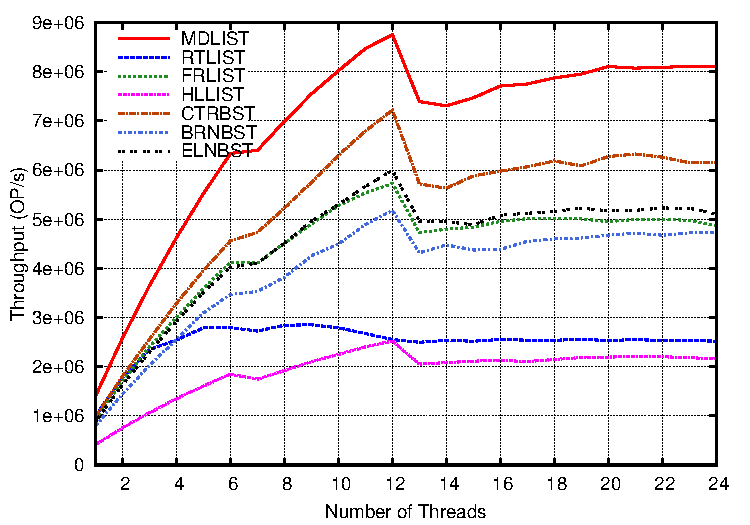
\includegraphics[width=1\columnwidth]{./data/intel100ins4Bkey}
        \caption{4G keys, $100\%$ \textsc{Insert}}
        \label{fig:4g100ins}
    \end{subfigure}
    \hfill
    \begin{subfigure}{0.32\textwidth}
        \centering
        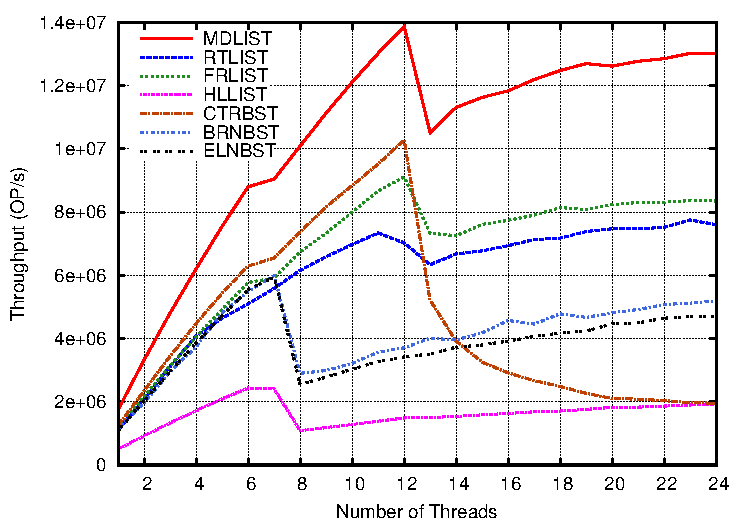
\includegraphics[width=1\columnwidth]{./data/intel30ins4Mkey}
        \caption{4M keys, $50\%$ updates}
        \label{fig:4m30ins}
    \end{subfigure}
    \hfill
    \begin{subfigure}{0.32\textwidth}
        \centering
        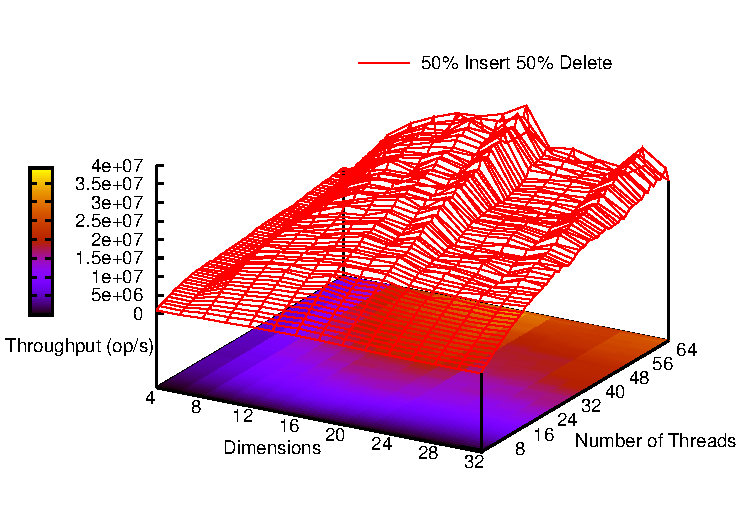
\includegraphics[width=1\columnwidth]{./data/amdsweep50ins}
      \caption{Dimension sweep}
        \label{fig:sweep}
    \end{subfigure}
    \caption{Throughput on SMP system and dimension sweep on NUMA}
    \label{fig:intel}
    \vspace{-0.2in}
\end{figure*}

Figures~\ref{fig:1k50ins},~\ref{fig:1m50ins} and~\ref{fig:1b50ins} depicted the write-dominated situation.
We observe that the both skiplist-based and BST-based dictionaries were able to explore fine-grained parallelism and exhibit similar scalability trends.
The overall throughput increases almost linearly until 16 threads, and continues to increase at a slower pace until 64 threads.
Because executions beyond 16 threads span across multiple chips, the performance growth is slightly reduced due to the cost of remote memory accesses.
The executions are no longer fully concurrent beyond 64 threads, thus the overall throughput is capped and may even reduce due to context switching overhead.
For small key space of 1K keys (Figure~\ref{fig:1k50ins}, RCU-based Citrus trees stand out against the rest.
This is because most insertions would not update the data structures due to the existence duplicated keys, and they essentially become read-only operations for which RCU is optimized.
MDLIST has slightly larger overhead for traversing operations if it is under-populated. 
To locate an existing node, the prefix matching algorithm always needs to perform $D$ comparison operations, whereas in a BST, the search algorithm could terminate much earlier because of shallow depth.
For 1M key space (Figure~\ref{fig:1m50ins}, most approaches achieve similar throughput except for HLLIST.
MDLIST outperform the other approaches by an average of $25\%$.
It continues to excel in large key space with one billion keys.
As shown by Figure~\ref{fig:1b50ins}, MDLIST outperforms the best alternatives including FRLIST and CTRBST by as much as $100\%$. 
For larger key space, insertions are less likely to collide with an existing key.
The size of the data structures grows much quicker too.
Each insertion in MDLIST modifies at most two consecutive nodes, incurring less remote memory access than the skiplist-based and BST-based approaches.

Figures~\ref{fig:1k20ins},~\ref{fig:1m20ins} and~\ref{fig:1b20ins} show the throughput for the mixed workload.
The overall scalability trends for all three key ranges mimic those of the write-dominated workload respectively.
In key spaces with 1M to 1G keys, MDLIST achieves $15\%~30\%$ speedup over FRLIST and ELNBST, which are two of the best skiplist-based and BST-based algorithms in mixed workload.
Figures~\ref{fig:1k9ins},~\ref{fig:1m9ins} and~\ref{fig:1b9ins} show the throughput for the read-dominated workload.
As the distribution of mutating operations further decreases to one tenth of the whole operations, the performance gaps among different algorithms begin to diminish.
For 1G keys (Figure~\ref{fig:1b9ins}, RTLIST, FRLIST, CTRBST, and ELNBST have almost identical performance up until 8 threads.
This is because all the data structures being tested implement logarithmic search.
Less writes means less interference between concurrent updates and traverse.
The performance characteristics of difference algorithms thus converge towards an ideal straight line.
They differ only in term of scalability at high levels of concurrency.
CTRBST achieves the best scalability among the alternatives but is still $20\%$ slower than MDLIST.
Note that in Figure~\ref{fig:1k9ins} CTRBST's performance degrades drastically when the benchmark spawn more threads than the number of available hardware cores.
CTRBST employs a user level RCU library that uses global locks, which may delay running threads if the threads holding the locks get preempted.

%When we increase the dimensionality of MDPQ to 16, we obtain on average a $50\%$ throughput gain over 8DPQ.
%A 16DPQ contains at most 4 nodes in each dimension.
%In order to reach the target position the search operation traverses a maximum of 64 nodes comparing to 128 nodes in a 8DPQ.
%Further increases in dimensionality can result in diminishing returns for concurrent \textsc{Insert}.
%The growing number of child pointers causes synchronization overhead that cancels the benefit of having less nodes in each dimension.



Figure~\ref{fig:4g100ins} and~\ref{fig:4m30ins} show the throughput of the algorithms on the SMP system.
The $x$-axis in these graphs is in linear scale.
In Figure~\ref{fig:4g100ins}, the executions consist solely of \textsc{Insert} operations, which insert keys in the range of 32-bit integers.
For all approaches, the overall system throughput peaks at 12 threads which is the maximum number of hardware threads.
Executions beyond 12 threads are preemptive, and the throughput slightly dropped due to unbalanced load causing increasing amount of cache invalidation.
MDLIST provides an average of $30\%$ speedup over CTRBST on all levels of concurrency.
While the performance of the BST-based approaches closely resembles each other, the performance of skiplist-based approaches varies.
Notably, the throughput of RTLIST drops significantly beyond 6 threads.
The impact of a dedicated maintenance is clearly visible on the SMP system, where the background thread has to compete with working threads for limited hardware cores.
Because the background thread is the only thread that does physical deletion, the overall progress will stagnate once the it is suspended.
In Figure~\ref{fig:4m30ins}, we distribute the workload by having $30\%$ insertions, $20\%$ deletions and $50\%$ searches.
MDLIST outperforms FRLIST by as much as $60\%$.
The throughput of CTRBST again drops drastically after exhausting all hardware threads.

In Figure~\ref{fig:sweep}, we sweep the dimension of MDLIST from 4 to 32 on the NUMA system, and show that the algorithm achieves maximum throughput with 20 dimensions on 64 threads. 
On all scale levels, we see that the throughput converges towards 20 dimensions.
This means that the way the dimensionality of an MDLIST affects its performance is independent from the number of threads.
The performance of MDLIST can be optimized if the access pattern of the user application is taken into account.
%The parametric sweep also reveals that the overall throughput is capped with 20 threads.
%This implies that the algorithms with inherent sequential semantics, such the \textsc{DeleteMin} operation, pose scalability challenges for NUMA systems.

Overall, MDLIST excels at high levels of concurrency with large key spaces.
The locality of its operations makes it suitable for NUMA architectures where remote memory access incurs considerable performance penalties.
On an SMP system with low concurrency, MDLIST performs equally well or even better than the state of the art skiplist-based and BST-based approaches.

\section{Related Work}
\label{sec:related}
Concurrent key-value store data structures that implement abstract dictionaries have been extensively studied in the literature.
Unordered dictionaries can be built upon non-blocking hash tables~\cite{michael2002high}, which achieve $\mathcal{O}(1)$ amortized cost.
Range queries are not attainable on such data structures because keys are not totally ordered.
We thus focus our discussion on BSTs and skiplists, which provide totally ordered key-value store and logarithmic search time by retaining balance either explicitly or probabilistically.
%Unlike simpler data structures such as arrays and linked lists, which already have highly efficient non-blocking implementations~\cite{harris2001pragmatic,herlihy2012art}, maintaining the balance invariants introduces synchronization overhead and contention.
%A great deal of research effort has been put into  
%While these approaches differ on the exact details of synchronization

\subsection{Search Trees}
%Early concurrent BSTs~\cite{guibas1978dichromatic,kung1980concurrent,nurmi1991uncoupling} are mostly lock-based adaptations of the sequential data structures, which focused on decoupling update and rebalancing to explore coarse-grained parallelism.
%The strict balance invariants were relaxed in the sense that the balancing condition can be temporarily violated by updates and eventually restored by subsequent rebalancing operations.
Recent fine-grained locking implementations by Bronson et al.~\cite{bronson2010practical} and Afek et al.~\cite{afek2012cbtree} take advantage of optimistic concurrently control and hand over hand validation to reduce synchronization overhead. 
The lock-based relaxed AVL tree by Crain et al.~\cite{crain2013contention} further reduces contention by delaying tree rotation and employing a dedicated maintenance thread to remove logically deleted nodes.
Drachsler et al.~\cite{drachsler2014practical} proposed a relaxed balanced and an unbalanced lock-based BSTs in which the nodes store additional logical ordering data by pointing to its logical predecessor and successor.
The search operation would traverse the logical chain to locate the target if it does not find the target after reaching a physical leaf node.
In comparison, the proposed MDList has deterministic physical layout pertaining to the logical ordering, which allows for more straightforward and efficient search operations.
%Nevertheless, locks are blocking.
%If a thread stalls while holding a lock, then other threads may have to wait for extended periods of time.

%Non-blocking algorithms avoid the pitfalls of locks by using powerful synchronization primitives such as \textsc{compare-and-swap} (CAS)~\cite{herlihy2012art}.
%Two widely adopted non-blocking progress guarantees are: lock-freedom, and wait-freedom.
%Lock-freedom ensures system wide progress while allowing individual threads to starve~\cite{herlihy2012art}.
%Whereas wait-freedom guarantees fair progress for every single thread~\cite{herlihy2012art}.
%Universal constructions~\cite{herlihy1993methodology,barnes1993method,chuong2010universal,fatourou2011highly} can be used to derive non-blocking BSTs but precludes concurrency due to the general nature of these methods. 
%For example, Herlihy's construction~\cite{herlihy1993methodology} requires that each thread only makes modification to a local copy of the data structure and updates the pointer to it using atomic operations.
%This serves as a fault tolerance scheme to avoid deadlocks rather than exploit fine-grained parallelism.
%Software transactional memory (STM)~\cite{herlihy2003software} can also be applied to obtain concurrent BSTs, e.g. the relaxed red-black trees proposed by Fraser~\cite{fraser2007concurrent} and Crain et al.~\cite{crain2012speculation}.
%However, like universal constructions, they are easily vanquished by carefully tailored locking and non-blocking schemes due to high STM overhead.

%Valois~\cite{} outlined a possible design of node-oriented non-blocking BST using CAS without giving full details.
Fraser~\cite{fraser2004practical} presented a non-blocking BST using multi-word CAS, which is not available on existing multi-core chips and expensive to implement using CAS. 
The first practical lock-free linearizable BST design was given by Ellen et al.~\cite{ellen2010non}.
Their implementation was based on a leaf-oriented BST, where values are stored externally in leaf nodes and internal nodes were only used for routing.
%Lock-freedom is achieved by using co-operative technique proposed by Barnes~\cite{barnes1993method} and Turek et al.~\cite{turek1992locking}.
Howley and Jones~\cite{howley2012non} presented a lock-free node-oriented BST based on the same co-operative technique.
Their algorithm has faster search operations than those in Ellen et al.'s algorithm because the search path is generally shorter in a node-oriented BST than in a leaf-oriented one.
On the other hand, Ellen et al.'s \textsc{Delete} operations, which avoid removing nodes with two children, are simpler and faster at the price of extra memory for internal nodes.
Natarajan and Mittal~\cite{natarajan2014fast} proposed a lock-free leaf-oriented BST, which marks edges instead of nodes.
Their algorithm is more efficient than previous approaches because the mutating operations work on a smaller portion of the tree and execute fewer atomic instructions.
Due to the complexity of rebalancing mentioned in Section~\ref{sec:intro}, all of the above non-blocking trees are not balanced, thus they subject to potential linear runtime for certain inputs.
Brown et al.~\cite{brown2014general} proposed a general template for implementing lock-free linearizable down-trees.
In order to orchestrate rebalancing among threads, their tree update routine atomically replaces a subgraph with a new connected subgraph using a set of multi-word synchronization primitives.
As recognized by the above researches, non-blocking rebalancing presents the biggest challenge to practical non-blocking BSTs.
The proposed MDList eliminates the need of balancing resulting in simpler and more efficient synchronization mechanisms.

%Later the approach is extended to the design of a lock-free $k$-ary tree~\cite{brown2011non} .  and Patricia tries~\cite{}

\subsection{Skiplists}
Pugh~\cite{pugh1990concurrent} designed a concurrent skiplist with per-pointer locks, where an update to a pointer must be protected by a lock. 
Shavit~\cite{shavit1999scalable} discovered that the highly decentralized skiplist is suitable for shared-memory systems and presents a concurrent priority queue based on Pugh's algorithm. 
In practice, probabilistic balancing is easier to implement and as efficient as deterministic balancing.
This is why the concurrent map class of the Java standard library uses skiplists rather than search trees~\footnote{http://www.java2s.com/Code/Java/Collections-Data-Structure/ConcurrentSkipListMap.htm}.
Fraser~\cite{fraser2004practical} proposed a lock-free skiplist with an epoch based memory reclamation technique.
It also employs the logical deletion technique, which was originally proposed by Harris~\cite{harris2001pragmatic}, to mark pointers and delay physical removal.
%Fomitchev and Ruppert~\cite{fomitchev2004lock} sketched a lock-free skiplist design but did not offer any implementation.
Sundell and Tsigas~\cite{sundell2004scalable} presented a provably correct linearizable lock-free skiplist, which uses exponential back-off to alleviate contention.
They guarantee linearizability by forcing threads to help physically remove a node before moving past it.
Herlihy et al.~\cite{herlihy2006provably} proposed an optimistic concurrent skiplist that simplifies previous work and allows for easy proof of correctness while maintaining comparable performance.
% Removed due to space constraint
%They later presented a optimistic skiplist~\cite{herlihy2007simple} that uses hand-over-hand locking to lock two nodes at a localized positions.
Crain et al.~\cite{crain2013no} proposed a no hot spot skiplist that alleviates contention by localizing synchronization at the least contended part of the structure.
Dick et al.~\cite{dick2014logarithmic} recently presented an improvement over existing skiplists algorithms.
Their lock-free skiplist uses rotating wheels instead of the usual towers to improve locality of reference and speedup traversals.
Skiplists have also been used to built a number of hybrid data structures.
Spiegel et al.~\cite{spiegel2010lock} combined a skiplist and a B-tree to produce a lock-free multi-way search tree, improving spatial locality of reference of skiplists by storing several elements in a single node.

\subsection{Tries}
Prokopec et al.~\cite{prokopec2012concurrent} proposed a lock-free hash array mapped trie using both single-word and double-word CAS.
They introduce intermediate nodes to solve the synchronization issue of updating the branching nodes.
However, the intermediate nodes also become hot spots for contention because every expansion of a branching node requires a new branching node to be linked to the corresponding intermediate node through CAS.
Oshman and Shavit~\cite{oshman2013skiptrie} proposed the lock-free skiptrie using double-word CAS, which combines a shallow skiplist with a x-fast trie to store high level nodes.
The MDList also bears some similarity to above mentioned tries in that the keys are ordered by their prefixes: a node always shares the same key prefix with its parent nodes.
The major difference lies in the partition strategies: in a trie a node shares the same prefix with all of its children, but in an MDList a node shares prefixes of different lengths with each of its child. 
This leads to a constant branch factor for nodes in tries and reducing branching factors for bottom levels nodes in MDLists.
Besides, retrieving the minimal key in a trie requires repetitive search, while MDList behaves like a heap where the root node always holds the smallest key.
Memory wise, the values are stored in a trie's leaf nodes, whereas they are stored in an MDList's internal nodes.

\section{Conclusion}
\label{sec:conclusion}
In this paper, we presented a simple and efficient lock-free dictionary design based on MDList.
It maps keys into high dimensional vector coordinates and achieve deterministic layout that is consistent with nodes' logical ordering.
We exploited spatial locality to increase the throughput of the \textsc{Insert} operations, and adopted asymmetrical logical deletion to address the synchronization overhead of the \textsc{Delete} operations.
When compared to the best available skiplist-based and BST-based algorithms, our algorithm achieved performance gains in scenarios with medium to large key spaces.
As much as $100\%$ performance improvement is achieved on a 64-core NUMA system, and an average of $40\%$ on a 12-core SMP system.
The performance of our dictionary can be tailored to different access patterns by changing its dimensionality.
We plan to improve the functionally of the dictionary by implementing concurrent range queries and iterator operations.
%Furthermore, our algorithm provides a scalable alternative to skiplists and search trees, which opens up opportunities for implementing other multiprocessor data structures, such as priority queues and sparse vectors.

\bibliographystyle{IEEEtran}
\bibliography{citation}

\end{document}
